
\subsection{\secState{R}Chaotic Reach set}\label{s:chaoticReachSet}

\paragraph{Motivation:} Design of calculation method for \emph{Reach Set Approximation} guarantying high \emph{Maneuverability}.

\paragraph{Background:}There is \emph{Coverage Ratio} property of \emph{Reach Set} (def. \ref{def:coverageRatio}). It has been shown that creating \emph{Reach Set} via \emph{greedy approach} is not feasible due the \emph{Scaling Factor}.  \emph{Contracted Expansion} (sec. \ref{s:constrainedTrajectoryExpansion}) is enabling to apply selection criteria while building \emph{Reach Set} in given \emph{Cell}. 

The \emph{Cell} $cell_{i,j,k}$ has a center and walls from UAS viewpoint: front wall , back wall (for $layer > 1$), top wall, left wall, right wall, bottom wall. It is expected that trajectory leading close to one cell walls will continue to different cell, increasing chance to obtain more \emph{Unique Footprints}. 

\paragraph{Expansion Constraint Function Implementation} (alg. \ref{alg:ExpansionConstraintFunctionForChaoticReachSet}) is based on simple principle: \emph{Select candidate Nodes which are  closest to outer walls of Cell, with unique footprint}.

\paragraph{Tuning Parameters}: \emph{Proximity to Cell outer wall} gives good chances to break into other rows or columns in \emph{Avoidance Grid}. \emph{Unique footprint} guarantees future \emph{Unique Footprint} after appending Trajectory by \emph{Movement application}. 
\begin{enumerate}
    \item \emph{Considered Footprint Length} - how much last cells in footprint should be considered in unique path track, minimal value 1, default value 3, maximal value $\infty$. If you want to generate non redundant trajectories use $\infty$, it will consider full footprint.
    
    \item \emph{Spread Limit} - upper limit of candidates which are going to be select for further expansion, minimal value 1, default value \emph{Count of unique Moves in Movement set}, maximal value $\infty$. If more than default values is selected the algorithm will generate \emph{redundant trajectories}. If less is selected then some trajectories are omitted and \emph{Coverage Rate} decreases sharply. 
\end{enumerate}


\paragraph{Step: Initialization} initialization of \emph{candidate} array (return value), \emph{leftovers} array (return Value). Node array \emph{passing} is populated with \emph{Nodes} which represents \emph{end node of Trajectory} and the tip of \emph{trajectory is constrained in \emph{cell}$_{i,j,k}$}.

\paragraph{Step: Evaluate best trajectories with unique Footprints} following steps are executed:
\begin{enumerate}
    \item \emph{Best Performance Map} is created with \emph{footprint} as key set element to ensure footprint uniqueness.
    \item \emph{Wall distance} for \emph{test node} is calculated as a closest trajectory portion distance to \emph{top, bottom, left, right} wall of cell $cell_{i,j,k}$
    \item \emph{Footprint} for \emph{test node} is created with maximal length given by \emph{Footprint Length} tuning parameter.
    \item \emph{Existence and Performance Test} is executed to ensure that best performing node is selected. If there is not key entry in the \emph{Best Performance Map}, then new entry for \emph{Test Node} is created. If there is key entry, the performance of \emph{Old Node} and \emph{Test Node} is compared and better is stored.
\end{enumerate}

\paragraph{Step: Select candidates} is executed on \emph{Best Performance Map} records using  \emph{Wall distance} as pivot parameter, ordering by closest proximity and limited by \emph{Search Limit} tuning parameter. The \emph{Leftovers} are difference set between \emph{Passing Nodes} and \emph{Candidate Nodes}. 

\begin{algorithm}[H]
    \SetKwInOut{Input}{Input}\SetKwInOut{Output}{Output}\SetKwInOut{TuningParameters}{Tuning Parameters}
    \Input{Node[] stack, Cell cell$_{i,j,k}$}
    \TuningParameters{int$^+$ footprintLength, int$^+$ spreadLimit}
    \Output{Node[] candidates, Node[] leftovers}
    
    \BlankLine
    \# Initialize structures\;
    Node[] candidates = [], Node[] leftovers=[]\;
    Node[] passing = cell$_{i,j,k}$.getFinishingTrajectories(stack)\;
    
    \BlankLine
    \# Select best performing trajectories with unique footprint\;
    Map$<$Footprint,Node$>$  bestPerformanceMap\;
    \For{Node test $\in$ passing}{
        wallDistance= test.minimalDistanceToWall(cell$_{i,j,k}$)]\;
        footPrint = test.getFootprint(lastCells = footprintLength)\;
        \eIf{bestPerformanceMap.contains(footPrint)}{
            old = bestPerformanceMap.getByKey(footprint)\;
            oldPerformance= old.minimalDistanceToWall(cell$_{i,j,k}$)\;
            \If{oldPerformance $>$ wallDistance}{
                bestPerformanceMap.setByKey(footprint,test)\;         
            }
        }{
            bestPerformanceMap.setByKey(footprint,test)\;
        }
    }
    
    \BlankLine
    \# Select best performing nodes up to \emph{spreadLimit} count\;
    candidates = bestPerformanceMap.select(count = spreadLimit).orderBy('wallDistance','Ascending')\;
    leftovers = passing - candidates\;
    \Return{[candidates,leftovers]}
    
    
    \caption{Expansion Constraint function for \emph{Chaotic Reach Set Approximation}}
    \label{alg:ExpansionConstraintFunctionForChaoticReachSet}
\end{algorithm}

\paragraph{Example:} for \emph{Avoidance Grid} with \emph{Distance 10 m}, \emph{Layer count 10}, \emph{Horizontal range $[-45^\circ,+45^\circ]$}, \emph{Horizontal Cell Count 7}, \emph{Vertical range $[-30^\circ,+30^\circ]$}, and \emph{Vertical Cell Count 5}. Is given in (fig. \ref{fig:chaoticReachSetApproximation}). The UAS is at \emph{Back-side} of \emph{Figure} (initial state is at all \emph{Trajectory Origins}). The \emph{black dashed line} marks \emph{Avoidance Grid} space boundary. Each trajectory has its own color and ends at \emph{Front-side} of \emph{Avoidance Grid Boundary}.


\begin{figure}[H]
    \centering
    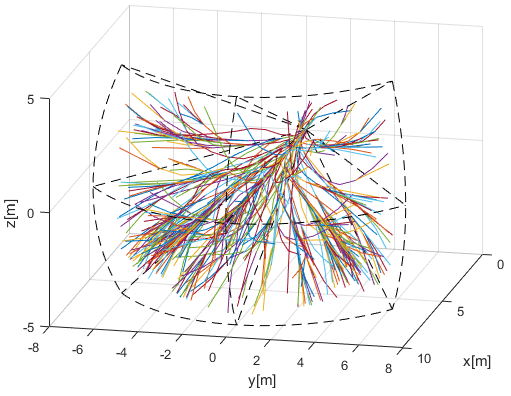
\includegraphics[width=0.7\linewidth]{\FIGDIR/RS002ChaoticReachSetEstimationMethod} 
    \caption{\emph{Chaotic \emph{reach set} approximation}.}
    \label{fig:chaoticReachSetApproximation}
\end{figure}

\paragraph{Pros and Cons:} It can be seen from example (fig. \ref{fig:chaoticReachSetApproximation}) that \emph{Chaotic Reach Set Approximation Method} (alg. \ref{alg:ExpansionConstraintFunctionForChaoticReachSet}) generates a lot of \emph{turning} and \emph{shaky} \emph{trajectories}. 

\emph{High Coverage Ratio} ($\sim 0.9$) is provided, while keeping \emph{medium node count}. The calculation complexity scales linearly with grid size. The \emph{upper limit of trajectories} is given as follow:

\begin{multline}
    countTrajectories(ReachSet) \le layerCellCount \times spreadLimit\\ \times size(Movements)
\end{multline}

\noindent The \emph{upper limit of nodes} is given as follow:
    
\begin{multline}
    countNodes(ReachSet) \le layerCount \times  layerCellCount  \\
    \times size(Movements) \times spreadLimit  
\end{multline}

\noindent\emph{Absence} of \emph{Smooth Trajectories} disqualifies \emph{Chaotic Reach Set Approximation} to be used for \emph{Navigation}. This type of reach set is feasible for \emph{Avoidance}, because it contains variety of maneuvers.


\subsection{\secState{R}Harmonic Reach set}\label{s:harmonicReachSet}

\paragraph{Motivation:} Imagine having an \emph{Avoidance Grid} like (fig. \ref{fig:LidarSpaceSegmentation}). There is a need of \emph{Reach Set Approximation} which will have \emph{Smooth Trajectories} (def. \ref{def:SmoothnessRatingForTrajectory}) going nearby $cell$ centers.

\paragraph{Background:} The \emph{Smoothness Rating for Trajectory} (def. \ref{def:SmoothnessRatingForTrajectory}) uses two distinct sets \emph{Smooth Movements} and \emph{Chaotic Movements} (eq. \ref{eq:ChaoticSmoothMovementSetDefinition}) which are defined for our \emph{Movement Automaton}  (sec. \ref{s:modelMAImplementation}) like follow:

\begin{equation}
    \begin{aligned}
    Smooth Movements &= \{Straight\} \\
    Chaotic Movements &= Movements - Smooth Movements\\
    \end{aligned}
\end{equation}

\emph{Smooth Movements} contains only \emph{Straight} movement, because others are considered as extreme turning movements. \emph{Smooth Movements} should contain only direct flight movements or slight heading correction. \emph{Chaotic Movements} set is supplement of \emph{Movement Automaton`s Movement Set}. 

The \emph{Avoidance Grid} (fig. \ref{fig:LidarSpaceSegmentation}) cell centers for fixed indexes $j_{fix}$, $k_{fix}$ are linearly aligned with \emph{initial state}. That means that  cell centers of cells $cell_{1,j_{fix},k_{fix}},\dots, cell_{i,j_{fix},k_{fix}}$, where $i$ is count of \emph{layers} lies on one line.  If the trajectory can achieve \emph{cell center} on some \emph{layer} only minor trajectory corrections are required to stay on given line. This type of trajectory gives us following advantages:
\begin{enumerate}
    \item\emph{Minimal steering at beginning} - the minimal steering is advantageous in \emph{Controlled Airspace} because is diminishing the amount of communication to \emph{UTM Service}.
    
    \item\emph{Additional safe space in Linear segment} - once the \emph{center of cell} is reached, \emph{Trajectory} sticks to line between cell centers. Each point on this line has \emph{maximal distance} to outer walls of cell. This gives us extra space given as minimum of distance between \emph{UAS position} and \emph{Outer cell walls}.
\end{enumerate}

\paragraph{Expansion Constraint Function Implementation} (alg. \ref{alg:ExpansionConstraintFunctionForHarmonicReachSet}) is based on simple principle: \emph{Select candidate Nodes  which are closest to Cell center, with unique footprint}.

\begin{note}
    \emph{Cell center} can be closely reached by \emph{smooth movement} from previous cell or \emph{chaotic movement} from neighbouring cell from current or previous layer. These trajectories are usually equivalent in \emph{Smoothness}.
\end{note}

\paragraph{Tuning Parameter:} \emph{Proximity to Cell Center} gives a good chance to keep trajectory smooth or \emph{smooth after one correction maneuver}. It has been mentioned that \emph{Cell Center} can be reached by various trajectories. In this method full footprint length is always considered, therefore only one tuning parameter can be offered:
\begin{enumerate}
    \item \emph{Spread Limit} - upper limit of candidates which are going to be selected for further expansion, minimal value 1, default value \emph{Count of unique Moves in Movement set}, maximal value $\infty$. If maximal value $\infty$ is selected, algorithm will generate skeleton of \emph{Reach Set} with full Coverage and with the smoothest \emph{Trajectories}.
\end{enumerate}

\paragraph{Step: Initialization} sets candidate \emph{Nodes} as empty set, leftover \emph{Nodes} as empty set. and selects all \emph{Nodes} from \emph{Stack} which represents  \emph{Finishing Trajectories} in working cell $cell_{i,j,k}$.

\paragraph{Step: Evaluate smoothest trajectories with unique Footprints} is implemented as \emph{multi-criteria filtration}. 

\emph{First criterion} is \emph{distance to Cell Center} which is penalized by trajectory \emph{smoothness rate} implemented in method \emph{Node.getPerformance(Cell $cell_{i,j,k}$)} defined as follow.

\begin{equation}
    getPerformance(Node,Cell) = \frac{distance(Node.Trajectory,Cell.Center)}{SmoothnessRate(Node.Trajectory)}
\end{equation}

\noindent Distance of \emph{Trajectory} is \emph{enumerator}, because its considered as \emph{base value} and is defined in interval $[0,maximalWallDistance]$. The \emph{Smoothness Rate} is in denominator, because it is a penalization coefficient defined in interval $[0,1]$. 

\emph{Second criterion} is \emph{trajectory uniqueness} This is provided by \emph{Best Performance Map}, where best performing \emph{Node} belongs to one unique \emph{trajectory footprint}. The implementation is identical to \emph{chaotic reach set expansion} (alg. \ref{alg:ExpansionConstraintFunctionForChaoticReachSet}).

\paragraph{Step: Select candidates} is executed  on \emph{Best Performance Map} records using \emph{Penalized Cell Center Distance} as pivot parameter, ordered in ascending order and limited by \emph{Spread Limit} tuning parameter. The \emph{Leftovers} are difference set between \emph{Passing Nodes} and \emph{Candidate Nodes}.

\begin{algorithm}[H]
\SetKwInOut{Input}{Input}\SetKwInOut{Output}{Output}\SetKwInOut{TuningParameters}{Tuning Parameters}
    \Input{Node[] stack, Cell cell$_{i,j,k}$}
    \TuningParameters{int$^+$ spreadLimit}
    \Output{Node[] candidates, Node[] leftovers}
    
    \BlankLine
    \# Initialize structures\;
    Node[] candidates = [], Node[] leftovers=[]\;
    Node[] passing = cell$_{i,j,k}$.getFinishingTrajectories(stack)\;
    
    \BlankLine
    \# Select unique smoothest trajectories\;
    Map$<$Buffer,Node$>$  bestPerformanceMap\;
    \For{Node test $\in$ passing}{
        centerDistance= test.getPerformance(cell$_{i,j,k}$)]\;
        footPrint = test.getFootprint()\;
        \eIf{bestPerformanceMap.contains(footPrint)}{
            old = bestPerformanceMap.getByKey(footprint)\;
            oldPerformance= old.getPerformance(cell$_{i,j,k}$)\;
            \If{oldPerformance $>$ centerDistance}{
                bestPerformanceMap.setByKey(footprint,test)\;         
            }
        }{
            bestPerformanceMap.setByKey(footprint,test)\;
        }
    }
    
    \BlankLine
    \# Select best performing nodes up to \emph{spreadLimit} count\;
    candidates = bestPerformanceMap.select(count = spreadLimit).orderBy('cellCenterDistance','Ascending')\;
    leftovers = passing - candidates\;
    \Return{[candidates,leftovers]}
    
    
    \caption{Expansion Constraint function for \emph{Harmonic Reach Set Approximation}}
    \label{alg:ExpansionConstraintFunctionForHarmonicReachSet}    
\end{algorithm}


\paragraph{Example:} for \emph{Avoidance Grid} with \emph{Distance 10 m}, \emph{Layer count 10}, \emph{Horizontal range $[-45^\circ,+45^\circ]$}, \emph{Horizontal Cell Count 7}, \emph{Vertical range $[-30^\circ,+30^\circ]$}, and \emph{Vertical Cell Count 5}. Is given in (fig. \ref{fig:harmonicReachSetApproximation}). The UAS is at \emph{Back-side} of \emph{Figure} (initial state is at all \emph{Trajectory Origins}). The \emph{black dashed line} marks \emph{Avoidance Grid} space boundary. Each trajectory has its own color and ends at \emph{Front-side} of \emph{Avoidance Grid Boundary}. The \emph{Spread Limit} in this case was set to $9$ which is \emph{Size of the Movement Set}.

\begin{note}
    Please note \emph{Trajectories} are organized in bundles going around \emph{Cell Centers smoothly}. Most of the steering maneuvers are executed at the \emph{beginning} of \emph{Avoidance Grid}.
\end{note}

\begin{figure}[H]
    \centering
    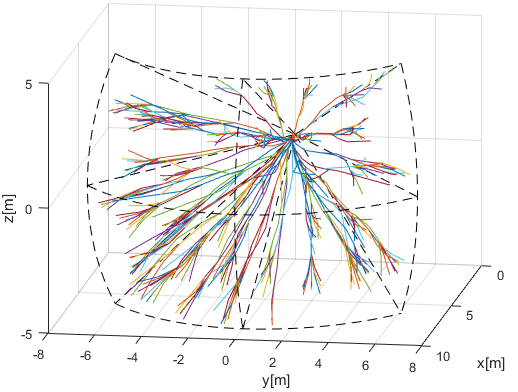
\includegraphics[width=0.7\linewidth]{\FIGDIR/RS003HarmonicReachSetEstimationMethod} 
    \caption{\emph{Harmonic \emph{reach set} approximation}.}
    \label{fig:harmonicReachSetApproximation}
\end{figure}

\paragraph{Pros and Cons:} It can bee seen from example (fig. \ref{fig:harmonicReachSetApproximation}) that \emph{Harmonic Reach Set Approximation Method} (alg. \ref{alg:ExpansionConstraintFunctionForHarmonicReachSet}) generates \emph{smooth evenly spread trajectories}.
    
High smoothness ratio ($\ge 0.9$) is provided, while keeping low node count for UAS systems. The calculation complexity scales linearly with grid size. The upper limit of trajectories is given as follow:

\begin{multline}
    countTrajectories(ReachSet) \le layerCellCount \times spreadLimit \\\times size(Movements)
\end{multline}

\noindent The \emph{upper limit of nodes} is given as follow:

\begin{equation}
    countNodes(ReachSet) \le layerCount \times layerCellCount \times spreadLimit
\end{equation}

\noindent Absence of \emph{High Coverage Ratio} disqualifies \emph{Harmonic Reach Set Approximation} to be used for \emph{Emergency Avoidance}. This type of \emph{Reach Set} is feasible for \emph{Open Space Navigation} or \emph{Controlled Airspace Navigation}. Its low turning rate in contained \emph{Trajectories} are desired for such tasks. 



\subsection{\secState{R}Combined Reach Set}\label{s:combinedReachSet}
\paragraph{Motivation:} Harmonic reach set (sec. \ref{s:harmonicReachSet}) is \emph{efficient} for \emph{Navigation in \emph{Controlled Airspace}}. Chaotic reach set (sec. \ref{s:chaoticReachSet}) is good for \emph{Emergency avoidance}. The need to differentiation between \emph{Navigation} and \emph{Emergency Avoidance} mode is necessary in \emph{Controlled Airspace}. but not in \emph{Non-controlled Airspace}. The combination of \emph{Harmonic} and \emph{Chaotic} reach sets is obvious solution. 

\emph{Automatic mode switch} can be provided by combination of \emph{Navigation Reach Set} and \emph{Avoidance Reach Set} with elevated cost function. Overall having a method to merge multiple trees would be beneficial.

\paragraph{Background:} If two \emph{Reach Set Approximation} were calculated for same \emph{Avoidance Grid} and \emph{Initial State}, using same \emph{Movement Automaton} and \emph{UAS model} are possible to merge. 

The \emph{Reach Set Approximation} is \emph{tree} with \emph{Root Node} in \emph{initail state} with movement buffer = $\varnothing$. The \emph{movement buffer} in each node can be used as \emph{route trace} during merging procedure. The example two reach set merge can be given as follow, where only \emph{latest} applied movement is taken into account.

\begin{equation}\label{eq:mergeTreeFunctionExample}
    \left[
    \begin{aligned}
    \texttt{Fi}&\texttt{rst Reach Set}\\
        &\varnothing \to 
            \left<
                \begin{aligned}
                    &left \to \left<
                                \begin{aligned}
                                    &left\\
                                    &right
                                \end{aligned}
                              \right.\\
                    &\varnothing\\
                \end{aligned}
             \right.\\ 
    \texttt{Se}&\texttt{cond Reach Set}\\
        &\varnothing \to 
            \left<
                \begin{aligned}
                    & \varnothing \\
                    & right \to \left< 
                                    \begin{aligned}
                                        &left\\
                                        &right
                                    \end{aligned}
                                \right.\\
                \end{aligned}
            \right.\\
    \end{aligned}
    \right]
    \to
    \left[
    \begin{aligned}
    \texttt{Co}&\texttt{mbined Reach Set}\\
    &\varnothing\to
        \left< 
            \begin{aligned}
                &left &\to   \left< 
                                \begin{aligned}
                                    &left\\
                                    &right
                                \end{aligned}    
                            \right.\\
                &right &\to   \left< 
                                \begin{aligned}
                                    &left\\
                                    &right
                                \end{aligned}    
                            \right.\\
            \end{aligned}    
        \right.
    \end{aligned}
    \right]
\end{equation}

\emph{First Reach Set} contains two trajectories given by buffers \emph{\{left,left\}} and \emph{\{left,right\}}. \emph{Second Reach Set} contains two trajectories given by buffers \emph{\{right,left\}} and \emph{\{right,right\}}. The \emph{Combined Reach Set} contains all four trajectories.

\begin{note}
    The combined tree \cite{o1996log} does not need to have combined amount of original \emph{Reach Sets} trajectories. There can be \emph{Duplicity} which means that any bounded property like \emph{Cost} must be \emph{calculated} again.
\end{note}

\paragraph{Combined Reach Set Calculation Function} (alg. \ref{alg:ReachSetMerge}) is implemented as function $Node combinedReachSet(\dots)$ which takes root Node with \emph{initial State}, \emph{Avoidance Grid} and respective parameters for each calculation method. \emph{Harmonic spread} for \emph{Harmonic Reach set calculation} and \emph{Chaotic Spread}, \emph{Footprint Length} for \emph{Chaotic Reach set calculation}.

\emph{Separate Reach Sets} are calculated using \emph{Wave-front propagation} (alg. \ref{alg:Wavefront Propagation}) using respective \emph{Constrained Expansion} functions for \emph{Harmonic} (alg. \ref{alg:ExpansionConstraintFunctionForHarmonicReachSet}) and \emph{Chaotic} (alg. \ref{alg:ExpansionConstraintFunctionForChaoticReachSet}) reach sets.

\emph{Combined Reach Set} is created using \emph{Node mergeTree($\dots$)} function. Because different cost function or \emph{Bounded Parameters Calculation} may be applied on \emph{Original Reach Sets}.

\emph{Cost} for \emph{each node} needs to be recalculated due to original reach sets disparity. Function \emph{combined.applyCostFunction()} will recalculate the new cost for each node. 

The Goal is to have penalization for \emph{Chaotic behaviour}, implementation of \emph{Automatic Mode Switch} can be done like follows:
\begin{enumerate}
    \item \emph{Calculate Normal Cost} for Node $Cost(Node)$ for associated trajectory:\\ $Cost(Node.Trajectory)$.
    \item \emph{Calculate Penalization for \emph{Chaotic Behaviour}}, calculate \emph{Smoothness Rating for Trajectory} (def. \ref{def:SmoothnessRatingForTrajectory}) in interval $[0,1]$, introduce penalization with base $100 \%$.
\end{enumerate}

The final $Cost(Node)$ function is applied on each \emph{Combined Reach Set Node} and look like follows:

\begin{multline}
    Cost(Node) = Cost(Node.Trajectory) \times\dots\\\dots\times \left(1+ \left(1-SmoothnessRate(N ode.T rajectory)\right)\right)
\end{multline}

\paragraph{Merge Tree Function} $mergeTree(\dots)$ implements \emph{Outer Join} operation on two trees. Example was given in (eq. \ref{eq:mergeTreeFunctionExample}).
Function is applied on \emph{root Node} iterating over \emph{Movements in Movement Set}, because \emph{Movement is pivot}.

\begin{algorithm}[H]
    \SetKwProg{Fn}{}{}{}\SetKwFunction{FRecurs}{Node mergeTree}
    \SetKwProg{Fn}{}{}{}\SetKwFunction{FMain}{Node combinedReachSet}
    
    \BlankLine
    \# Tree merge function\;
    \Fn(){\FRecurs{Node firstNode, Node secondNode}}{
        \BlankLine
        \# Try to copy reference node or return null\;
        Node referenceNode = (firstNode?:(secondNode?: return null))\;
        Node merged =  new Node(referenceNode)\;
        merged.leafs= []\;
        \BlankLine
        \# Try to fetch movement nodes if exist in any sub tree\;
        \For{movement $\in$ Movements}{
            firstLeaf = firstNode.getLeafFor(movement)\;
            secondLeaf = secondNode.getLeafFor(movement)\;
            newLeaf = mergeTree(firstLeaf,secondLeaf)\;
            \If{newLeaf $\sim = $ null}{
                merged.leafs.append(newLeaf)\;
            }
        }
        \Return{merged}
    }{}
    
    \BlankLine
    \# Combined Reach Set calculation function\;
    \Fn(){\FMain{Node root, AvoidanceGrid grid,int$^+$ chaoticSpread, int$^+$ harmonicSpread, int$^+$ footprintLength}}{
        Node chaotic = chaoticReachSet(root,grid, footprintLength,chaoticSpread)\;
        Node harmonic = harmonicReachSet(root,grid, harmonicSpread)\;
        Node combined = mergeTree(chaotic,harmonic)\;
        combined.applyCostFunction()\;
        \Return{combined}
    }

    
    \caption{Reach Set Merge Function and Combined Reach Set calculation}
    \label{alg:ReachSetMerge}
\end{algorithm}

\paragraph{Example:} for \emph{Avoidance Grid} with \emph{Distance 10 m}, \emph{Layer count 10}, \emph{Horizontal range $[-45^\circ,+45^\circ]$}, \emph{Horizontal Cell Count 7}, \emph{Vertical range $[-30^\circ,+30^\circ]$}, and \emph{Vertical Cell Count 5}. Is given in (fig. \ref{fig:combinedReachSetApproximation}). The UAS is at \emph{Back-side} of \emph{Figure} (initial state is at all \emph{Trajectory Origins}). The \emph{black dashed line} marks \emph{Avoidance Grid} space boundary. Each trajectory has its own color and ends at \emph{Front-side} of \emph{Avoidance Grid Boundary}. The \emph{Chaotic Spread} was set to 8, \emph{Footprint Length} to 3 and \emph{Harmonic Spread} to 1.

\begin{note}
    Notice there are typical trajectories from both \emph{Harmonic} (fig. \ref{fig:harmonicReachSetApproximation}) and \emph{Chaotic} (fig. \ref{fig:chaoticReachSetApproximation}) \emph{Reach Set Approximations}.
\end{note}

\begin{figure}[H]
    \centering
    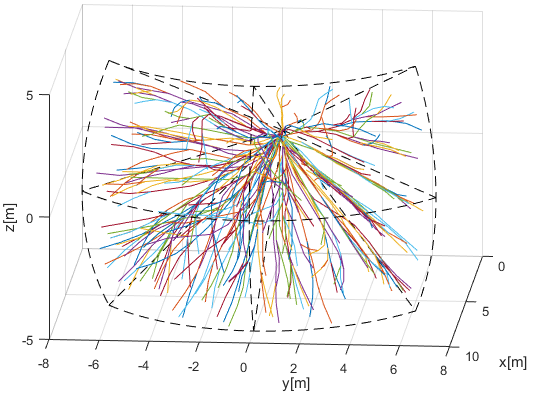
\includegraphics[width=0.7\linewidth]{\FIGDIR/RS004CombinedReachSetEstimationMethod} 
    \caption{\emph{Combined \emph{reach set} approximation}.}
    \label{fig:combinedReachSetApproximation}
\end{figure}


\paragraph{Pros and Cons:} It can bee seen from example (fig. \ref{fig:combinedReachSetApproximation}) that \emph{Combined Reach Set Approximation} (alg. \ref{alg:ReachSetMerge}) contains both types of maneuvers. \emph{Cheaper Smooth} for navigation and \emph{More Expensive Chaotic} for \emph{Emergency Avoidance}. The upper limit of trajectories is given as follow:

\begin{multline}
    countTrajectories(ReachSet) \le countTrajectories(Chaotic) \\+ countTrajectories(Harmonic)
\end{multline}

\noindent The \emph{upper limit of nodes} is given as follow:

\begin{equation}
    countNodes(ReachSet) \le countNodes(Chaotic)+ countNodes(Harmonic)
\end{equation}

\noindent \emph{Harmonic Reach Set} is ideal for \emph{Non-controlled Airspace} missions, because it contains \emph{Automatic Mode Switch} between \emph{Navigation} and \emph{Emergency Avoidance}.


\subsection{\secState{R}ACAS-X like Reach set}\label{s:acasReachSet}
\paragraph{Motivation:} The implementation of \emph{ACAS-Xu} behavior in DAA system will  be mandatory for \emph{National Airspace System Integration} in United spaces \cite{shively2018uas}. 

Implementation of ACAS-Xu like behaviour increase usability of approach, if it can be achieved without major concept changes.


\paragraph{Background:} The \emph{ACAS-Xu} system on operational level has been described in \cite{marston2015acas}. The \emph{Policy for Collision Avoidance} proposal has been given in \cite{julian2016policy}.

Some behavioural patterns can be encoded into  \emph{Reach Set}. ACAS-Xu navigation part is basically \emph{Look-up table of Maneuvers for Allowed Separations}.
 
The \emph{Evasive Maneuver} selection process in ACAS-Xu is similar to our approach: \emph{Select most energy efficient maneuver in compliance with space-time constraints}. ACAS-Xu intruder model is similar to our \emph{Body Volume Intersection Model} (sec. \ref{s:bodyvolumeIntersection}). The \emph{ACAS-Xu} defines following base separations:

\begin{enumerate}
    \item \emph{Horizontal} - movements on \emph{Horizontal Plane} in \emph{Global Coordinate System}.
    
    \item \emph{Vertical} - movements on \emph{Vertical Plane} in \emph{Global Coordinate System}.
    
\end{enumerate}

\noindent There are allowed custom separations which can be used, for further experimentation: 
\begin{enumerate}
    \item \emph{Slash} - movement on $+45^{\circ}$ \emph{Tilted Plane to Horizontal Plane} in \emph{Global Coordinate System}.
    
    \item \emph{Backslash} - movement on $-45^{\circ}$ \emph{Tilted Plane to Horizontal Plane} in \emph{Global Coordinate System}.
    
\end{enumerate}

\noindent For given \emph{Movement Automaton} implementation (sec. \ref{s:modelMAImplementation}) the separations are given as follow:

\begin{equation}\label{eq:implementedseparations}
    \begin{aligned}
        Horizontal & = \{Straight, Left, Right \}\\
        Vertical & = \{Straight, Up, Down\}\\
        Slash & = \{Straight, UpLeft, DownRight\}\\
        Backslash & = \{Straight, UpRight, DownLeft\}\\
    \end{aligned}
\end{equation}

\noindent For each $Node(\dots,buffer)$ and each \emph{separation} there is a evaluation function $isSeparation$ which decides, if \emph{Trajectory} defined by node buffer is made up only from \emph{Separation} movements.  The function $isSeparation(\dots)$ is defined like:

\begin{equation}\label{eq:isSeparationPredicate}
    isSeparation(buffer,separation) =
    \begin{cases}
        \begin{aligned}
            \forall & movement \in buffer,\\ & movement \in separation
        \end{aligned}&: true\\
        otherwise &: false
    \end{cases}
\end{equation}

Following \emph{Separation Modes} can be defined with given \emph{separations}:

\begin{enumerate}
    \item \emph{Horizontal} (ACAS-X defined mode) containing \emph{horizontal} separation. 
    
    \item \emph{Vertical} (ACAS-X defined mode) containing \emph{vertical} separation.
    
    \item \emph{Horizontal-Vertical} (ACAS-X defined mode) containing \emph{horizontal, vertical} separations.
    
    \item \emph{Full} (custom defined mode) containing all \emph{Separation Modes}.
    
\end{enumerate}

\begin{note}
    Every separation modes generates 2D trajectories set on \emph{Respective plane}. There is no need for \emph{Tuning parameters} for further \emph{Expansion Constraint}.    
\end{note}

\paragraph{Expansion Constraint Function Implementation} (alg. \ref{alg:ExpansionConstraintFunctionForACASLikeReachSet}) is based on simple principle:
\emph{Select only candidate Nodes which Trajectories have at least one desired Separation Mode}.

\paragraph{Step: Initialization} sets candidate \emph{Nodes} as empty set,  leftover \emph{Nodes} as empty set, and, select all nodes form \emph{stack} which represents \emph{Finishing Trajectories} in working $cell_{i,j,k}$,

\paragraph{Step: Candidate Selection Process} is evaluated for each \emph{test Node} from \emph{passing Node Set}. 

For each \emph{applicable separation}, given as input parameter \emph{separations}, The test function \emph{isSeparation} (eq. \ref{eq:isSeparationPredicate}) is applied:
\begin{enumerate}
    \item If \emph{test Node} trajectory belongs to at least one allowed separation it is added to candidates set.
    \item Else is added to \emph{Leftovers}.
\end{enumerate}

\begin{note}
    \emph{Separation sets} (eq. \ref{eq:implementedseparations}) are not \emph{exclusive sets} in \emph{Movement Automaton} domain. One \emph{Trajectory} contained by Node can belong to multiple \emph{Separations}.    
\end{note}

\begin{algorithm}[H]
\SetKwInOut{Input}{Input}\SetKwInOut{Output}{Output}\SetKwInOut{TuningParameters}{Tuning Parameters}
    \Input{Node[] stack, Cell cell$_{i,j,k}$, Separation[] separations}
    \TuningParameters{$None:\varnothing$}
    \Output{Node[] candidates, Node[] leftovers}
    
    \BlankLine
    \# Initialize structures\;
    Node[] candidates = [], Node[] leftovers=[]\;
    Node[] passing = cell$_{i,j,k}$.getFinishingTrajectories(stack)\;
    
    \BlankLine
    \# Select nodes containing trajectories with usable separations\;
    \For{Node test $\in$ passing}{
        \For{separation $\in$ separations}{
            \BlankLine
            \# Get separations for Node\;
            Separations[] nodeSeparations = test.getSeparations()\;
            \BlankLine
            \# If trajectory given by buffer is on Separation plane\;
            \If{isIn(isSeparation(test.buffer,separation)(\ref{eq:isSeparationPredicate})}{
                candidates.append(test)\;
            }
        }
        \BlankLine
        \# If there was no applicable separation, throw Node away\;
        \If{test $\not\in$ candidates}{
            leftovers.append(test)\;
        }
    }
    \BlankLine
    \# Return results\;
    \Return{[candidates,leftovers]}
    
    \caption{Expansion Constraint function for \emph{ACAS-like Reach Set Approximation}}
    \label{alg:ExpansionConstraintFunctionForACASLikeReachSet}    
\end{algorithm}

\paragraph{Example:} for \emph{Avoidance Grid} with \emph{Distance 10 m}, \emph{Layer count 10}, \emph{Horizontal range $[-45^\circ,+45^\circ]$}, \emph{Horizontal Cell Count 7}, \emph{Vertical range $[-30^\circ,+30^\circ]$}, and \emph{Vertical Cell Count 5}. Is given in (fig. \ref{fig:acasLikeReachSetVariousSeparationMode}). The UAS is at \emph{Back-side} of \emph{Figure} (initial state is at all \emph{Trajectory Origins}). The \emph{black dashed line} marks \emph{Avoidance Grid} space boundary. Each trajectory has its own color and ends at \emph{Front-side} of \emph{Avoidance Grid Boundary}.

\emph{Full} separation mode given in (fig. \ref{fig:acasLikeReachSetFull}). \emph{Horizontal-Vertical} separation mode, used in original \emph{ACAS-Xu} testing \cite{marston2015acas}, given in (fig. \ref{fig:acasLikeReachSetHorizontalVertical}). \emph{Horizontal} separation mode given in (fig. \ref{fig:acasLikeReachSetHorizontalOnly}) is usually used by planes. \emph{Vertical} separation mode given in (fig. \ref{fig:acasLikeReachSetVerticalOnly}) is usually used by copters.

\begin{figure}[H]
	\centering
    \begin{subfigure}{0.48\textwidth}
        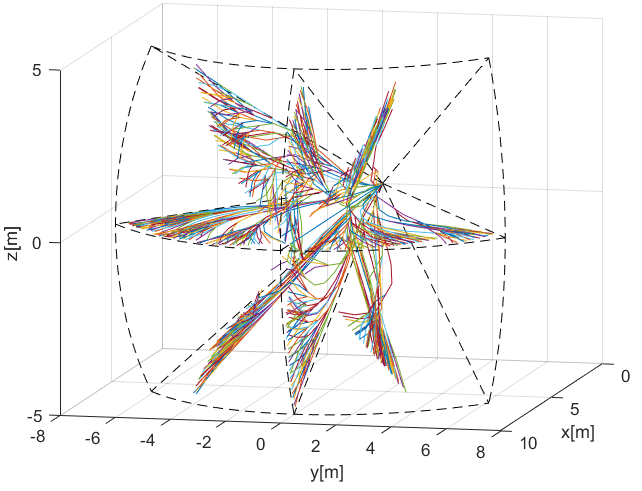
\includegraphics[width=0.9\linewidth]{\FIGDIR/RS005ACASLikeReachSetEstimationMethodFull}
        \caption{Full.}
        \label{fig:acasLikeReachSetFull}
    \end{subfigure}
    \begin{subfigure}{0.48\textwidth}
        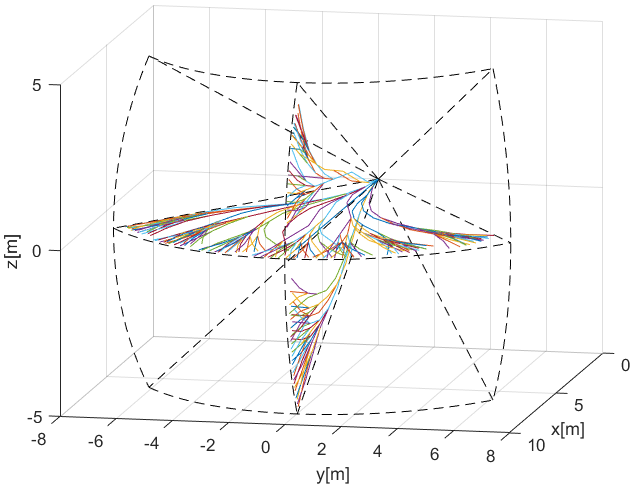
\includegraphics[width=0.9\linewidth]{\FIGDIR/RS006ACASLikeReachSetEstimationMethodHorizontalVertical} 
        \caption{Horizontal-Vertical.}
        \label{fig:acasLikeReachSetHorizontalVertical}
    \end{subfigure}
    \\
    \begin{subfigure}{0.48\textwidth}
        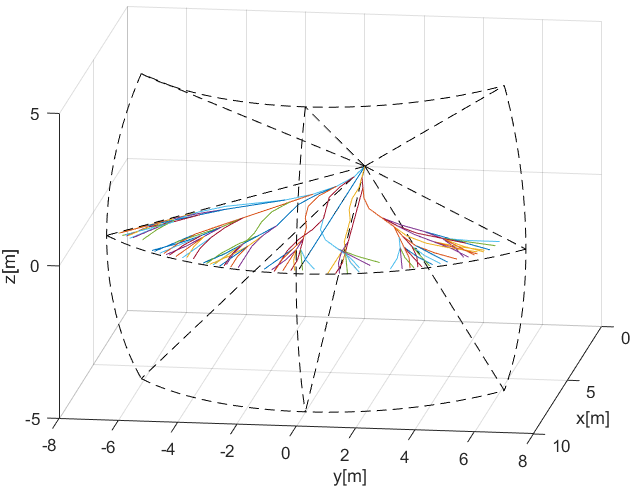
\includegraphics[width=0.9\linewidth]{\FIGDIR/RS008ACASLikeReachSetEstimationMethodHorizontal} 
        \caption{Horizontal.}
        \label{fig:acasLikeReachSetHorizontalOnly}
    \end{subfigure}
    \begin{subfigure}{0.48\textwidth}
        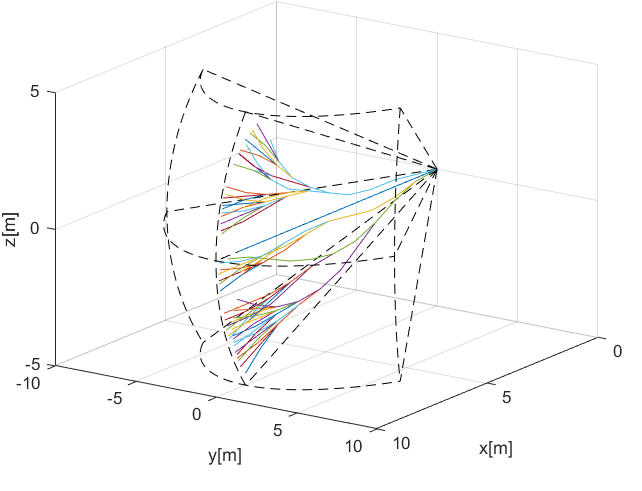
\includegraphics[width=0.9\linewidth]{\FIGDIR/RS009CASLikeReachSetEstimationMethodVertical} 
        \caption{Vertical.}
        \label{fig:acasLikeReachSetVerticalOnly}
    \end{subfigure}
    \caption{ACAS-X imitation \emph{reach set} approximation for various \emph{separation modes}. }
    \label{fig:acasLikeReachSetVariousSeparationMode}
\end{figure}

\paragraph{Pros and Cons:} It can be seen from examples (fig. \ref{fig:acasLikeReachSetVariousSeparationMode}) that \emph{ACAS-like Reach Set Approximation Method} (alg. \ref{alg:ExpansionConstraintFunctionForACASLikeReachSet}) generates full reach set for 2D plane located in 3D space. 

The \emph{Reach Set} contains trajectories with \emph{high coverage ratio} and \emph{high smoothness rating} for selected 2D separation plane. Overall performance compared to full 3D reach sets (sec. \ref{s:chaoticReachSet}, \ref{s:harmonicReachSet} \ref{s:combinedReachSet}) is poor. 

The \emph{node} and \emph{trajectory} count boundary was not implemented. It is common knowledge that \emph{2D} avoidance sets does not require scaling \cite{marston2015acas}. Otherwise trajectory footprint mechanism like in \emph{Harmonic Reach Set Approximation} (alg. \ref{alg:ExpansionConstraintFunctionForHarmonicReachSet}) can be introduced.

This reach set implements \emph{Planar-Separation} as native feature, it can be used for both \emph{navigation} and \emph{avoidance} tasks in \emph{Controlled Airspace}. For \emph{Non-controlled Airspace} there are far more superior \emph{Combined Reach Set} (sec. \ref{s:combinedReachSet}).
